\documentclass[a4paper,12pt]{article} % Tipo de documento y tamaño de letra.
\usepackage[utf8]{inputenc} % Para que reconozca caracteres especiales como tildes.
\usepackage[spanish, es-nodecimaldot]{babel} % Para definir el idioma y el formato de fechas en español.
\usepackage{amsmath, amssymb} % Paquetes para símbolos y ecuaciones avanzadas (Para hacer una ecuación con un recuadro).
\usepackage{ragged2e} % Para justificar textos.
\usepackage{multicol} % Para crear columnas.
\usepackage{slashed} % Para generar números o variables canceladas (Una línea diagonal sobre el número o variable).
\usepackage{graphicx} % Paquete para poner graficas.
\usepackage{float} % Para poder dejar la imagen en un punto fijo del documento.
\usepackage{longtable} % Para tablas largas.
\usepackage{cancel} % Para hacer cancelaciones en medio de operaciones.
\usepackage{xcolor} % Para el color y esas cosas.
\usepackage{apacite} % Paquete para citas APA.
\usepackage{fancyhdr} % Para personalizar encabezados y pies de página.
\usepackage{geometry} % Para ajustar márgenes.
\usepackage{setspace} % Para ajustar el interlineado.
\usepackage{natbib} % Para manejar las citas y que no queden pegadas y feas :P.
\usepackage{hyperref} % Para que los enlaces funcionen con su URL.
\usepackage[version=4]{mhchem}  % Versión recomendada para mayor funcionalidad.
\usepackage{chemfig} %También para hacer estructuras químicas.
\usepackage{array} % Para mejor control de las columnas.
\usepackage{siunitx} % Para unidades físicas.
\usepackage{tabularx}
\usepackage[table]{xcolor}
\usepackage{booktabs}

\pagestyle{fancy}
\fancyhf{} % Limpia encabezados y pies de página predeterminados
\fancyhead[L]{\textbf{EJERCICIOS SOBRE ÓPTICA.}} % Encabezado izquierdo
\fancyhead[R]{\textbf{ÓPTICA GEOMÉTRICA.}} % Encabezado derecho
\fancyfoot[C]{\thepage} % Número de página en el centro del pie

\geometry{headheight=12.96115pt, top=1in, bottom=1in, left=1in, right=1in}
\begin{document}


\begin{figure}[H]
	\centering
	
\includegraphics[width=0.5\textwidth]{Unir.jpg}
\end{figure}

\vspace{\baselineskip}


\begin{center}
	\textbf{\Large } \\[0.3cm]
	\vspace{\baselineskip}
	\textbf{} \\[0.4cm]
	\textbf{Grado en Física.} \\[0.8cm]
	\textbf{Liz Ángel Núñez Torres.} \\[1 cm]
	\textbf{Universidad Internacional de La Rioja.} \\[1 cm]
	\textbf{1 de Abril 2026.}
\end{center}

\newpage
\tableofcontents

\newpage

\begin{itemize}
	\item \textbf{Al lector:}
	\begin{justify}
		Para hacer más cómoda la lectura del archivo, se ha optado por colorear de \textcolor{orange}{naranja} los resultado parciales y de color \textcolor{blue}{azul} los resultado definitivos.
	\end{justify}
\end{itemize}

\section{Tubo de vidrio lleno de acetaldehído.}

\begin{justify}
	Se tiene un tubo de vidrio de grosor despreciable, lleno de acetaldehído (n=1.35). 
	En su extremo está cerrado por una superficie esférica de 25 cm de radio, convexo 
	hacia el aire que lo rodea. Determinar: 
\end{justify}

\begin{enumerate}
	\item Distancias focales objeto e imagen. 
	\item Imagen de un objeto situado a 1 m. ¿Cómo es la imagen? 
	\item Imagen de un objeto situado a 60 m. ¿Cómo es la imagen? 
\end{enumerate}

\vspace{\baselineskip}

\begin{justify}
	\textbf{Datos:}
\end{justify}

\begin{multicols}{3}
	\(n_1 = 1.35.\)

	\(n_2 = 1.\)

	\(R = 25 \, cm.  \)
\end{multicols}

\begin{justify}
	Como la superficie es convexa hacia el aire, visto desde el interior, es decir, del acetaldehído hacia el aire, el radio que se forma 
	es positivo.
\end{justify}

\begin{justify}
	Para obtener las distancias focales usaremos la \textbf{ecuación del dioptrio esférico.}
\end{justify}

\[ \textcolor{orange}{\boxed{ - \frac{n_1}{x} + \frac{n_2}{x'} = \frac{n_2 - n_1}{R}.}} \]

\subsection{Distancia focal objeto.}

\begin{justify}
	Por definición, los ángulos no convergen y la imagen se produce desde el infinito. Por lo tanto nuestra ecuación es:
\end{justify}

\[ -\frac{n_1}{x} + \cancel{\frac{n_2}{\infty}} = \frac{n_2 - n_1}{R}. \]

\begin{justify}
	Sustituimos:
\end{justify}

\[ -\frac{n_1}{x} = \frac{n_2 - n_1}{R} \Rightarrow -\frac{1.35}{x} = \frac{1 - 1.35}{25}. \]

\begin{justify}
	Despejando \(\mathbf{x}\) obtenemos:
\end{justify}

\[ x = -\frac{1.35}{\left(-0.014\right)}. \]

\vspace{\baselineskip}

\[\textcolor{blue}{\boxed{x = 96.42 \, cm.}}\]

\vspace{\baselineskip}

\subsection{Distancia focal imagen.}

\begin{justify}
	Por definición, los rayos del objeto vienen desde el infinito, por lo tanto tenemos que la ecuación es:
\end{justify}


\[ \cancel{-\frac{n_1}{\infty}} + \frac{n_2}{x'} = \frac{n_2 - n_1}{R}. \]

\begin{justify}
	Sustituimos:
\end{justify}

\[ -\frac{n_2}{x'} = \frac{n_2 - n_1}{R} \Rightarrow \frac{1}{x'} = \frac{1 - 1.35}{25}. \]

\begin{justify}
	Despejando \(\mathbf{x'}\) obtenemos:
\end{justify}

\[ x' = -\frac{1}{\left(0.014\right)}. \]

\vspace{\baselineskip}

\[\textcolor{blue}{\boxed{x' = -71.42 \, cm.}}\]

\vspace{\baselineskip}

\subsection{Objeto a un metro.}

\begin{justify}
	Para calcular la imagen que este objeto genera, usaremos de nuevo la \textbf{ecuación del dioptrio esférico.}
\end{justify}

\begin{justify}
	Donde \( x = 100 \, cm\).
\end{justify}

\[  -\frac{1.35}{100} + \frac{1}{x'} = \frac{1 - 1.35}{25}. \]

\begin{justify}
	Despejando \(x'\) tenemos:
\end{justify}

\[ x' = - \frac{1}{5 \times 10^{-4}} = -2000 \, cm \]

\vspace{\baselineskip}

\[ \textcolor{blue}{\boxed{ x' = -20 \, m.}} \]

\vspace{\baselineskip}

\subsection{Objeto a sesenta metros.}

\begin{justify}
	Definimos \(x = 6000 cm\) y procedemos de nuevo con la ecuación del dioptrio esférico.
\end{justify}

\[  -\frac{1.35}{6000} + \frac{1}{x'} = \frac{1 - 1.35}{25}. \]

\begin{justify}
	Despejando \(x'\).
\end{justify}

\[ x' = \frac{1}{1.42 \times 10^{-2}} = -72.64 \, cm. \]

\vspace{\baselineskip}

\[ \textcolor{blue}{\boxed{ x' = -0.726 m.}} \]

\vspace{\baselineskip}

\subsection{¿Cómo son las imágenes?}

\begin{justify}
	Para saber como son las imágenes vamos a usar la ecuación del \textbf{aumento lateral.}
\end{justify}

\[ \beta = \frac{n_1 \cdot x}{n_2 \cdot x'}. \]

\begin{itemize}
	\item Imagen para un objeto a un metro.
\end{itemize}

\[ \beta_1 = \frac{1.35 \cdot (-20)}{1 \cdot 1}. \]

\vspace{\baselineskip}

\[ \textcolor{orange}{\boxed{\beta_1 = -27.}} \]

\vspace{\baselineskip}

\begin{justify}
	\centering
	\textcolor{blue}{La imagen es virtual, invertida y aumentada.}	
\end{justify}

\vspace{\baselineskip}

\begin{itemize}
	\item Imagen para un objeto a sesenta metros.
\end{itemize}

\[ \beta_2 = \frac{1.35 \cdot (-0.726)}{60 \cdot 1}. \]

\vspace{\baselineskip}

\[ \textcolor{orange}{\boxed{\beta_2 = -0.0163.}} \]

\vspace{\baselineskip}

\begin{justify}
	\centering
	\textcolor{blue}{La imagen es virtual, invertida y disminuida.}	
\end{justify}

\vspace{\baselineskip}

\section{Esfera de vidrio inmersa en el agua.}

\begin{justify}
	Estamos inmersos en una piscina llena de agua (n=1.33) y tenemos una esfera de vidrio
	(n=1.5) de radio 8 cm. En el centro de dicha esfera se encuentra un objeto pequeño. 
	Determinar la posición de la imagen, aumento lateral y naturaleza de la imagen.
\end{justify}

\begin{justify}
	Como el objeto es real es positivo, la distancia es de \(8 \, \mathrm{m}\), dado que está en el centro de la esfera.
\end{justify}

\vspace{\baselineskip}

\subsection{Posición de la imagen.}

\begin{justify}
	Usaremos nuevamente la \textbf{ecuación del diotrio esférico} con el radio negativo debido que se mide la distancia a partir del polo del dioptrio esférico.
\end{justify}

\[- \frac{1.5}{8} + \frac{1.33}{x'} = \frac{1.33 - 1.5}{-8}. \]

\begin{justify}
	Despejamos \( \mathbf{x'}\).
\end{justify}

\[ \textcolor{blue}{\boxed{x' = 6.37 \, \mathrm{cm}.}} \]

\vspace{\baselineskip}

\subsection{Aumento lateral.}

\begin{justify}
	Ssustituimos en la ecuación nuestros datos:
\end{justify}

\[ \beta = \frac{1.5 \cdot 6.37}{1.33 \cdot 8}. \]

\vspace{\baselineskip}

\[\textcolor{blue}{\boxed{\beta = 0.900. }}\]

\vspace{\baselineskip}

\subsection{Naturaleza de la imagen.}

\begin{justify}
	Con los datos obtenidos, podemos argüir:
\end{justify}

\vspace{\baselineskip}

\begin{justify}
	\centering
	\textcolor{blue}{La imagen es real, derecha y reducida.}	
\end{justify}


\vspace{\baselineskip}

\section{Espejo convexo.}

\begin{justify}
	Detrás de un espejo convexo de 20 cm de radio de forma una imagen virtual a 5 cm. Determinar:
\end{justify}

\begin{itemize}
	\item Distancias focales objeto e imagen.
	\item Posición del objeto.
	\item Recalcular las distancias focales y la posición del objeto si se tuviera un espejo cóncavo. 
	\item Naturaleza de la imagen en ambos casos.
\end{itemize}

\vspace{\baselineskip}

\subsection{Distancia focal objeto e imagen (Espejo convexo).}

\begin{justify}
	Recordemos que estamos usando el convenio paraxial, por lo tanto para un \textbf{espejo convexo (divergente)} el radio y la distancia focal son:
\end{justify}

\begin{multicols}{2}
	\[\mathrm{R < 0}.\]
	
	\[\mathrm{f < 0}.\]
\end{multicols}

\vspace{\baselineskip}

\begin{justify}
	Para calcular la distancia focal usaremos:
\end{justify}

\[ \textcolor{orange}{\boxed{f = \frac{R}{2}.}} \]

\vspace{\baselineskip}

\begin{justify}
	Antes de calcularlo, debemos recordar que en un espejo las distancias focales objeto e imagen coinciden en el mismo punto porque los rayos se reflejan.
\end{justify}

\vspace{\baselineskip}

\[ \textcolor{orange}{ \boxed{f_{objeto} = f_{imagen}.}} \]

\vspace{\baselineskip}

\begin{justify}
	Sustituyendo el radio, tenemos entonces que la distancia focal es:
\end{justify}

\[ f = \frac{-20}{2}. \]

\vspace{\baselineskip}

\[ \textcolor{blue}{\boxed{f = -10 \, \mathrm{cm}.}} \]

\vspace{\baselineskip}

\subsection{Posición del objeto (Espejo convexo).}

\vspace{\baselineskip}

\begin{justify}
	Usamos la ecuación de los espejos.
\end{justify}

\[ \frac{1}{x} + \frac{1}{x'} = \frac{1}{f}. \]

\begin{justify}
	Sustituimos:
\end{justify}

\[ \frac{1}{x} - \frac{1}{5} = \frac{1}{-10}. \ \]

\begin{justify}
	Despejamos:
\end{justify}

\[ \textcolor{blue}{\boxed{x = 10 \, \mathrm{cm}.}} \]

\vspace{\baselineskip}

\subsection{Distancia focal objeto e imagen (Espejo cóncavo.)}

\begin{justify}
	Para un \textbf{espejo cóncavo (convergente)} el radio y la distancia focal:
\end{justify}

\begin{multicols}{2}
	\[\mathrm{R > 0}.\]
	
	\[\mathrm{f > 0}.\]
\end{multicols}

\begin{justify}
	La distancia focal es entonces.
\end{justify}

\[ f = \frac{20}{2}. \]

\vspace{\baselineskip}

\[ \textcolor{blue}{\boxed{f = 10 \, \mathrm{cm}.}} \]

\begin{justify}
	Recordamos que las distancias focales objeto e imagen serán iguales.
\end{justify}

\vspace{\baselineskip}

\subsection{Posición del objeto (Espejo  cóncavo).}

\begin{justify}
	Usamos la ecaución de los espejos.
\end{justify}

\[ \frac{1}{x} + \frac{1}{-5} = \frac{1}{10}. \]

\begin{justify}
	Despejamos.
\end{justify}

\[ \textcolor{blue}{\boxed{x = 3.33 \, \mathrm{cm}.}} \]

\vspace{\baselineskip}

\subsection{Naturaleza de la imagen.}

\begin{itemize}
	\item Espejo convexo.
\end{itemize}

\begin{justify}
	Calculamos el aumento lateral.
\end{justify}

\[ \beta = -\frac{(-5)}{10}. \]

\[ \textcolor{orange}{\boxed{ \beta = 0.5 }}\]

\begin{justify}
	Por lo tanto la naturaleza de la imagen (recordemos que para un espejo la imagen siempre es virtual):
\end{justify}

\begin{justify}
	\centering
	\textcolor{blue}{Imagen virtual, derecha y disminuida.}
\end{justify}

\vspace{\baselineskip}

\begin{itemize}
	\item Espejo cóncavo.
\end{itemize}

\begin{justify}
	Calculamos el aumento lateral.
\end{justify}

\[ \beta = -\frac{(-5)}{3.33}. \]

\[ \textcolor{orange}{\boxed{ \beta = 1.5 }}\]

\begin{justify}
	Por lo tanto la naturaleza de la imagen.
\end{justify}

\begin{justify}
	\centering
	\textcolor{blue}{Imagen virtual, derecha y aumentada.}
\end{justify}

\vspace{\baselineskip}

\section{Cristalino visual.}

\begin{justify}
	El cristalino (n=1.65) de nuestros ojos es equivalente a una lente biconvexa cuyos radios varían para 
	enfocar la imagen en la retina. Entre ambos se sitúa el humor vítreo para el cual se asumirá que n=1. 
	La función del cristalino es enfocar la imagen en la retina, la cual se encuentra a 3 cm de distancia, 
	cuando el objeto esté tanto en el infinito como a 25 cm del ojo variando su radio. 
	Determinar el valor del radio del cristalino cuando el objeto está en el infinito y a 25 cm.
\end{justify}

\vspace{\baselineskip}

\begin{justify}
	Dado que tenemos una lente biconvexa, se cumple que:
\end{justify}

\begin{multicols}{2}
	\[ \mathrm{R}_1 > 0 .\]

	\[\mathrm{R}_2 < 0. \]
\end{multicols}

\begin{justify}
	Por lo que la luz incide en dioptrio convexo y refracta en un dioptrio cóncavo.
\end{justify}

\begin{justify}
	Para obtener el radio usaremos la \textbf{ecuación de la lente delgada} dado que el humor vítreo y el aire poseen el mismo índice de refracción.
\end{justify}

\[ \frac{1}{f} = \left(n - 1\right) \cdot \left(\frac{1}{R_1} - \frac{1}{R_2}\right). \]

\begin{justify}
	Y como definimos antes, \(R = R_1\) y \( R = -R_2\).
\end{justify}

\[ \frac{1}{f} = \left(n - 1\right) \cdot \left(\frac{1}{R} + \frac{1}{R}\right) \Rightarrow \frac{1}{f} = \left(n - 1 \right) \cdot \left(\frac{2}{R}\right). \]

\vspace{\baselineskip}

\[ \frac{1}{f} = \frac{2\left(2-1\right)}{R}. \]

\vspace{\baselineskip}

\[\textcolor{orange}{\boxed{R = 2\left(n-1\right)f.}}\]

\subsection{Objeto en el infinito.}

\begin{justify}
	Para obtener el radio cuando el objeto está en el infinito, usamos la \textbf{ecuación de las lentes delgadas} para obtener 
\end{justify}

\[ \frac{1}{3} + \cancel{\frac{1}{\infty}} = \frac{1}{f} \Rightarrow f = \frac{1}{\frac{1}{3}}. \]

\vspace{\baselineskip}

\[ \textcolor{orange}{\boxed{f = 3 \, \mathrm{cm}.}} \]

\vspace{\baselineskip}

\begin{justify}
	Usando la ecuación del radio que despejamos previamente, sustituimos por nuestros valores:
\end{justify}

\[ R = 2 \cdot \left(1.35 - 1\right) \cdot 3  \]

\vspace{\baselineskip}

\[ \textcolor{blue}{\boxed{R = 3.98 \, \mathrm{cm}.}} \]

\vspace{\baselineskip}

\subsection{Objeto a veinticinco centímetros.}

\begin{justify}
	Usando de nuevo la ecuación de lente delgadas tenemos:
\end{justify}

\[ \frac{1}{3} + \frac{1}{25} = \frac{1}{f} \Rightarrow f = \frac{1}{\frac{1}{3} + \frac{1}{25}}. \]

\vspace{\baselineskip}

\[\textcolor{orange}{\boxed{f = 2.67 \, \mathrm{cm}.}}\]

\vspace{\baselineskip}

\begin{justify}
	Reemplazamos este valor en nuestra ecuación del radio.
\end{justify}

\[ R = 2 \cdot \left(1.65 - 1\right) \cdot 2.67. \]

\vspace{\baselineskip}

\[ \textcolor{blue}{\boxed{R = 3.47 \, \mathrm{cm}.}} \]

\vspace{\baselineskip}

\begin{justify}
	El radio es mayor cuando el objeto está en el infinito que al estar a 25 cm.
\end{justify}

\vspace{\baselineskip}

\section{Lente convergente.}

\begin{justify}
	5.	Un objeto de altura 5 cm se encuentra delante de una lente convergente de distancia focal 30 cm.
	Detrás de dicha lente se quiere posicionar una pantalla para proyectar la imagen. Determinar:
\end{justify}

\begin{itemize}
	\item Posición de la pantalla para que se proyecte la imagen tal que esta tenga una altura cinco veces mayor que el objeto (la imagen debe ser real para poder ser proyectada). 
	\item Si detrás de la lente convergente se sitúa en contacto otra lente, ¿qué potencia debe tener esta para que la imagen tenga el doble de altura que el objeto? ¿Cuál debe ser la posición de la pantalla? 
\end{itemize}

\begin{justify}
	Recordemos que al ser convergente se cumple que:
\end{justify}

\begin{multicols}{2}
	\[R > 0.\]

	\[f > 0.\]
\end{multicols}

\vspace{\baselineskip}

\subsection{Posición para una imagen cinco veces mayor.}

\begin{justify}
	Usamos la formula del \textbf{aumento lateral}. Sabemos que la imagen real es \textbf{invertida}, por lo tanto.
\end{justify}

\[ \beta = -\frac{x'}{x}.\]

\begin{justify}
	Como queremos que sea cinco veces mayor, será invertido.
\end{justify}

\[ -5 = -\frac{x'}{x} \Rightarrow x' = 5x. \]

\begin{justify}
	como \(x'\) representa la imagen, usaremos el valor despejado en la ecuación  de lentes delgadas.
\end{justify}

\[ \frac{1}{x} + \frac{1}{x'} = \frac{1}{f} \Rightarrow \frac{1}{x} + \frac{1}{5x} = \frac{1}{30}. \]

\begin{justify}
	Despejando.
\end{justify}

\[ x = \frac{180}{5}. \]

\vspace{\baselineskip}

\[\textcolor{blue}{\boxed{x = 36 \, \mathrm{cm}.}}\]

\begin{justify}
	Y usando la formula obtenida al despejar el aumento lateral.
\end{justify}

\[ x' = 5 \cdot 36. \]

\vspace{\baselineskip}

\[\textcolor{blue}{\boxed{x' = 180 \, \mathrm{cm}.}}\]

\vspace{\baselineskip}

\begin{justify}
	Por lo tanto, la pantalla se coloca a 180 cm de distancia de la lente.
\end{justify}

\vspace{\baselineskip}

\subsection{Potencia para una imagen con el doble de altura.}

\begin{justify}
	Como tenemos la distancia focal, obtenemos la potencia de la primera lente.
\end{justify}

\[P_1 = \frac{1}{f} \Rightarrow \frac{1}{0.30}. \]

\vspace{\baselineskip}

\[ \textcolor{orange}{\boxed{P_1 = 3.33 \, \mathrm{D}.}} \]

\begin{justify}
	Para la doble altura del objeto, estando este a 36 cm de altura delante de la lente, siendo invertida y real.
\end{justify}

\[ \beta = - \frac{x'}{x} \Rightarrow -2 = - \frac{x'}{36}. \]
\vspace{\baselineskip}

\[\textcolor{blue}{\boxed{x' = 72 \, \mathrm{cm}.}}\]

\begin{justify}
	Una vez obtenemos la distancia de la imagen, podemos obtener la \textbf{distancia focal del sistema compuesto}. 
\end{justify}

\begin{justify}
	Para esto usamos la ecuación de las lentes delgadas.
\end{justify}

\[ \frac{1}{36} + \frac{1}{72} = \frac{1}{f} \Rightarrow f = \frac{1}{\frac{1}{36} + \frac{1}{72}}. \]

\vspace{\baselineskip}

\[\textcolor{orange}{\boxed{f = 24 \, \mathrm{cm}.}}\]

\begin{justify}
	Ahora con la distancia focal del sistema, obtenemos la potencia total del sistema.
\end{justify}

\[ P_T = \frac{1}{0.24}. \]
\vspace{\baselineskip}

\[\textcolor{orange}{\boxed{P_T = 4.16 \, \mathrm{D}. }}\]

\begin{justify}
	Con la potencia total del sistema y la potencia de la primera lente, obtenemos la potencia de la segunda lente.
\end{justify}

\[ P_T = P_1 + P_2 \Rightarrow P_2 = P_T - P_1 \Rightarrow P_2 = 4.16 - 3.33. \]

\[ \textcolor{blue}{\boxed{P_2 = 0.83 \, \mathrm{D}. }} \]

\begin{justify}
	\textbf{La posición de la pantalla y la potencia para que se cumpla la doble altura de la imagen es 0.83 D y 72 cm respectivamente.}
\end{justify}

\vspace{\baselineskip}

\section{Lente gruesa.}

\begin{justify}
	Una lente gruesa de vidrio (n=1.6) de 4 cm de grosor y radios R1=10 cm y R2=12 cm (ambas positivas) se encuentra inmersa en aire. Determinar:
\end{justify}

\begin{itemize}
	\item Distancia focal y potencia. 
	\item Posición de los planos principales primario y secundario y de los focos respecto a sus respectivos polos. 
	\item Para los radios dados, ¿es posible obtener \(P'e<0\) aumentando el espesor? 
\end{itemize}

\vspace{\baselineskip}

\subsection{Distancia focal.}

\begin{justify}
	La lente gruesa está inmersa en el aire, así que podemos usar la \textbf{ecuación del fabricante de lentes} para lentes gruesas.
\end{justify}

\[ \frac{1}{f} = \left(n-1\right) \left[\frac{1}{R_1} + \frac{1}{R_2} + \frac{\left(n-1\right)d}{n \, R_1 \, R_2}\right]. \]

\begin{justify}
	Sustituimos:
\end{justify}

\[ \frac{1}{f} = \left(1.6 - 1 \right) \left[\frac{1}{10} + \frac{1}{12} + \frac{\left(1.6-1\right)4}{1.6 \, 10 \, 12}\right]. \]

\begin{justify}
	Despejamos.
\end{justify}

\[ f = \frac{1}{0.6 \cdot 0.029}. \]

\vspace{\baselineskip}

\[\textcolor{blue}{\boxed{f = 57.14 \, \mathrm{cm}.}} \]

\vspace{\baselineskip}

\subsection{Potencia de la lente.}

\[P_T = \frac{1}{57.14} = 0.017 \, cm^{-1}.\]

\vspace{\baselineskip}

\[\textcolor{blue}{\boxed{P_T = 1.75 \, \mathrm{D}.}}\]

\vspace{\baselineskip}

\subsection{Planos principales primario y secundario.}

\begin{justify}
	Usamos la ecuación de los planos principales.
\end{justify}

\[ h = - \frac{f\left(n_2 - n_1\right)d}{R_2 \, n_2}. \]

\begin{itemize}
	\item \textbf{Principal primario.}
	
	\[h_1 = - \frac{57.14 \left(1.6-1\right)4}{12 \cdot 1.6}\]

	\[\textcolor{blue}{\boxed{h_1 = -7.14 \, \mathrm{cm}.}}\]

	\item \textbf{Principal secundario.}

	\[h_2 = - \frac{57.14 \left(1.6-1\right)4}{10 \cdot 1.6}\]

	\[\textcolor{blue}{\boxed{h_2 = -8.37 \, \mathrm{cm}.}}\]
\end{itemize}

\vspace{\baselineskip}

\subsection{Posición de los focos}

\begin{itemize}
	\item \textbf{Respecto a \(h_1\).}
	
	\[f = h_1 - f_T \Rightarrow -7.14 - 57.14\]

	\[\textcolor{blue}{\boxed{f = -64.28 \, \mathrm{cm}.}}\]

	\item \textbf{Respecto a \(h_2\).}
	
	\[f' = h_2 + f_T \Rightarrow -8.37 + 57.14\]

	\[\textcolor{blue}{\boxed{f' = 48,77 \, \mathrm{cm}.}}\]
\end{itemize}

\vspace{\baselineskip}

\subsection{¿Es posible una potencia negativa?}

\begin{justify}
	La potencia se obtiene de la forma:
\end{justify}

\[ P'e = P_1 + P_2 - d \, P_1 \, P2. \]

\begin{justify}
	Para calcular la potencia de cada superficie usaremos la ecuación de la \textbf{potencia de una esfera.}
\end{justify}

\[P = \frac{n_2 - n_1}{R}.\]

\begin{justify}
	Recordando que \(n_2\) y \(n_1\) son relativos a la lente, siguiendo el sistema paraxial.
\end{justify}

\begin{itemize}
	\item \textbf{Potencia de la primera lente.}
	
	\[ P_1 = \frac{1.6 - 1}{10}. \]

	\[ \textcolor{blue}{\boxed{P_1 = 0.06 \, \mathrm{D}.}} \]

	\item \textbf{Potencia de la segunda lente.}
	
	\[ P_2 = \frac{1 - 1.6}{12}. \]

	\[ \textcolor{blue}{\boxed{P_2 = -0.05 \, \mathrm{D}.}} \]
\end{itemize}

\begin{justify}
	La diferencia de signo entre \(P_1\) y \(P_2\) genera que el termino \(- d \, P_1 \, P2\) sea siempre positivo, debido a esto, si aumenta la distancia (espesor) será aun más positivo.
\end{justify}

\begin{justify}
	Por lo tanto, podemos afirmar que \(P'e < 0\) \textbf{no se cumple en nuestro caso.}
\end{justify}

\vspace{\baselineskip}

\section{Prisma de vidrio.}

\begin{justify}
	Un prisma de vidrio (n=1.55) delimitado por los puntos ABC, con ángulos A=25°, B=65°, C=90°, tiene el lado AB recubierto de un material reflectante. Determinar:
\end{justify}

\begin{itemize}
	\item Si se quiere un rayo que emerja perpendicular a la cara BC, el ángulo de incidencia en la cara AC.
	\item Desviación angular entre el rayo incidente y el transmitido. 
	\item Sin el material reflectante, ¿puede obtenerse la misma trayectoria anteriormente descrita?.
\end{itemize}

\subsection{Obtención de los ángulos.}

\begin{itemize}
	\item \textbf{Ángulo \(\theta_5\)}.
\end{itemize}

\begin{justify}
	Para obtener los ángulos, nos prestaremos atención a la siguiente imagen.
\end{justify}

\begin{figure}[H]
	\centering
	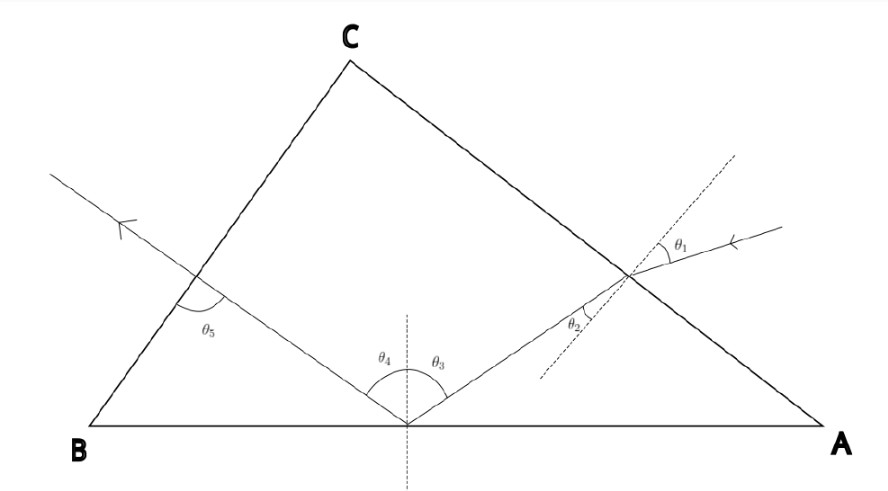
\includegraphics[width = 0.8 \textwidth]{fig1.jpg}
\end{figure}

\begin{justify}
	Como podemos apreciar, el rayo emergente por  \(\overline{BC}\) es congruente con la normal de esta cara, por lo tanto:
\end{justify}

\[\textcolor{orange}{\boxed{\theta_5 = 90^\circ}}\]

\begin{itemize}
	\item \textbf{Ángulo \(\theta_4\)}.
\end{itemize}

\begin{figure}[H]
	\centering
	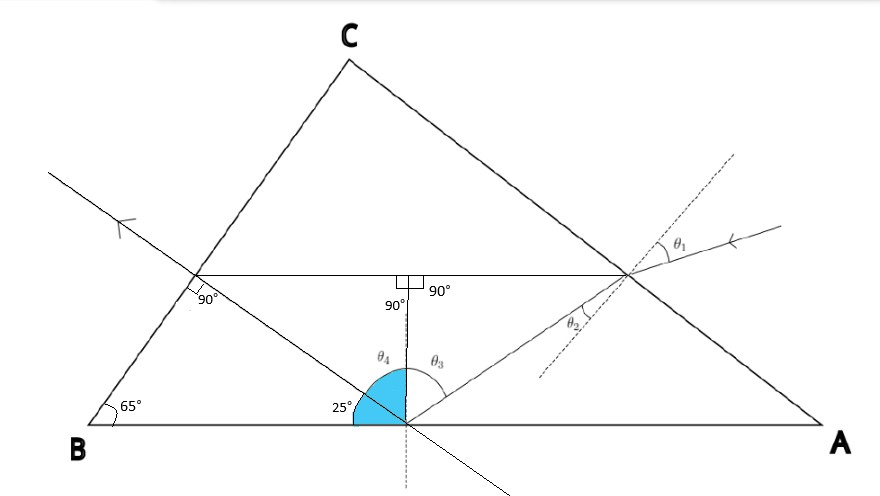
\includegraphics[width = 0.8 \textwidth]{fig2.jpg}
\end{figure}

\begin{justify}
	Como sabemos el valor del ángulo de \(B\) y de \(\theta_5\), podemos calcular la diferencia de \(180^\circ\) para el ángulo adyacente que se forma entre la cara \(\overline{BA}\) y la normal a la misma, \textbf{coloreado de azul}.
\end{justify}

\begin{justify}
	Esto tiene sentido porque el \textbf{rayo emergente} en la cara \(\overline{BC}\) es paralelo a \(\overline{CA}\) y como el ángulo de \textbf{A} es un \textbf{ángulo alterno externo}, ambos deben tener el mismo valor.
\end{justify}

\begin{justify}
	Es por esto que para obtener \(\theta_4\) sabemos que la normal en la cara \(\overline{BC}\) forma un ángulo de \(90^\circ\), así que \(\theta_4\) viene dado como:
\end{justify}

\[ 25^\circ + \theta_4 = 90^\circ. \Rightarrow \theta_4 = 90^\circ - 25^\circ. \]

\[\textcolor{orange}{\boxed{\theta_4 = 65^\circ.}}\]

\begin{itemize}
	\item \textbf{Ángulo \(\theta_3\)}.
\end{itemize}

\begin{figure}[H]
	\centering
	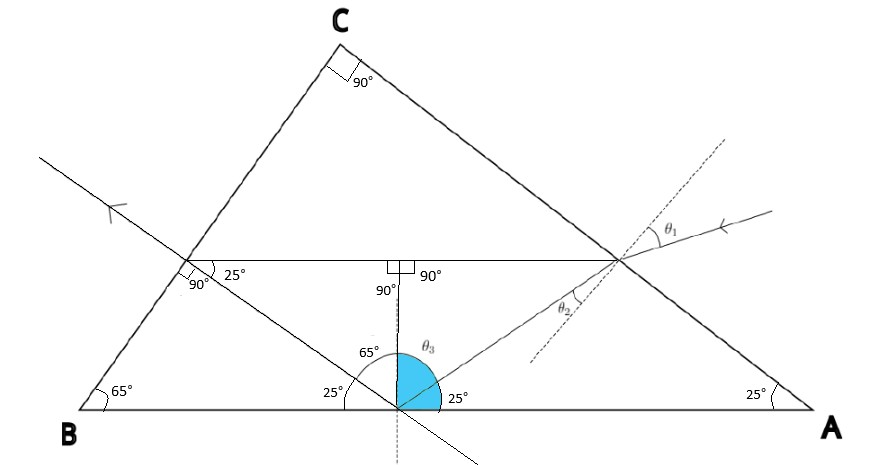
\includegraphics[width = 0.8 \textwidth]{fig3.jpg}
\end{figure}

\begin{justify}
	Es entonces que para obtener \(\theta_3\) primero obtendremos los \(25^\circ\) que son procendetes al ser un \textbf{ángulo opuesto por el vertice} del ángulo de \(25^\circ\) calculado anteriormente. Realizando el mismo procedimiento tenemos:
\end{justify}

\[\theta_3 = 90^\circ - 25^\circ.\]

\[\textcolor{orange}{\theta_3 = 65^\circ.}\]

\begin{justify}
	Que podemos rectificar al obtener \(180^\circ\) al sumar los ángulos coloreados de azul para este punto y el anterior.
\end{justify}

\begin{itemize}
	\item \textbf{Ángulo \(\theta_2\)}.
\end{itemize}

\begin{figure}[H]
	\centering
	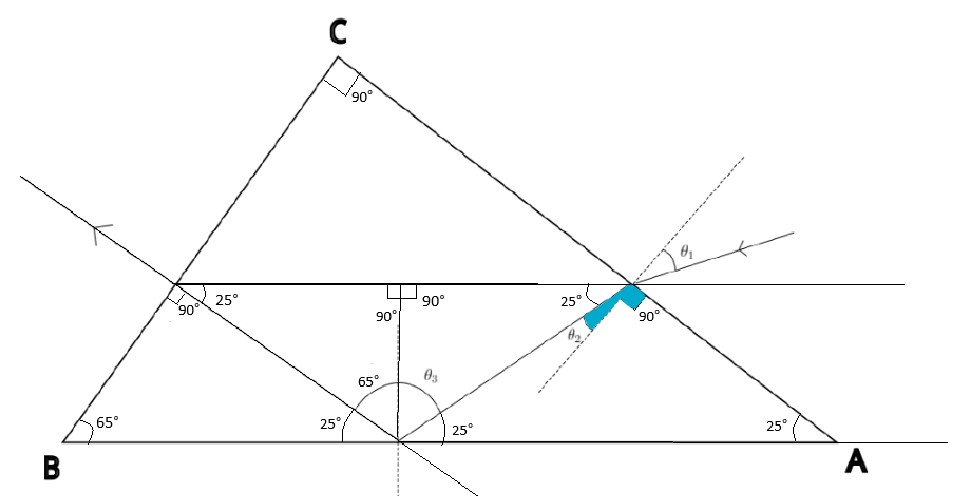
\includegraphics[width = 0.8 \textwidth]{fig4.jpg}
\end{figure}

\begin{justify}
	Finalmente, para calcular \(\theta_2\) buscamos una vez obtener una suma que correponda a \(180^\circ\), vemos que el ángulo superior coloreado es \(90^\circ + \theta_2\).
\end{justify}

\[ 25^\circ + 25^\circ + \left(90^\circ + \theta_2 \right) = 180^\circ.  \]

\[ 90^\circ + \theta_2 = 180^\circ - 50^\circ. \]

\[\theta_2 = 130^\circ  - 90^\circ.\]

\[\textcolor{orange}{\boxed{\theta_2 = 40^\circ.}}\]


\subsection{Ángulo de incidencia en AC.}

\begin{justify}
	Para obtener este ángulo usaremos la \textbf{ley de Snell.}
\end{justify}

\[ n_1 \cdot \sin(\theta_1) = n_2 \cdot \sin(\theta_1). \]

\begin{justify}
	Sustituimos.
\end{justify}

\[ 1.55 \cdot \sin(40) = 1 \cdot \sin(\theta_1). \]

\[ \theta_1 = \sin^{-1}(0.996). \]

\vspace{\baselineskip}

\[ \textcolor{blue}{\boxed{\theta_1 = 85.08^\circ.}} \]

\vspace{\baselineskip}

\subsection{Desviación angular.}

\begin{justify}
	La desviación angular corresponde al ángulo formado entre el ángulo por donde incide el rayo, en nuestro caso \(\theta_1\) y el ángulo emergente, en este caso \(\theta_5\). Como \(BC \perp AC\).
\end{justify}

\[ D = 90 - 85.08.\]

\[\textcolor{blue}{\boxed{D = 4.92^\circ.}}\]

\vspace{\baselineskip}

\subsection{Trayectoria del rayo sin el material reflectante en el prisma.}

\begin{justify}
	Sabemos que el ángulo formado por el rayo al incidir en la cara \(BA\) del prisma es de \(65^\circ\). 
\end{justify}

\begin{justify}
	Calculamos el ángulo crítico.
\end{justify}

\[\theta = \sin^{-1}\left(\frac{1}{n}\right).\]

\[ \sin^{-1}\left(\frac{1}{1.55}\right) \]

\vspace{\baselineskip}

\[\textcolor{blue}{\boxed{\theta = 40^\circ.}} \]

\begin{justify}
	Como el ángulo formado por el rayo al incidir en la cara \(BA\) es mayor que el ángulo crítico \(65^\circ > 40^\circ.\), se produce \textbf{reflexión total} en la superficie.
\end{justify}

\begin{justify}
	\centering
	\textcolor{blue}{Se obtiene la misma trayectoria sin el material reflectante.}
\end{justify}

\vspace{\baselineskip}

\section{Menisco positivo.}

\begin{justify}
	Un menisco positivo (\(R_1\)=5 cm, \(R_2\)=20 cm, n=1.5) se encuentra en contacto con una lente plano-convexo (\(R_2\)=-2 cm, n=1.6).  Considerando que ambas lentes son delgadas, determinar:
\end{justify}

\begin{itemize}
	\item Potencia y distancia focal del sistema equivalente.
	\item Potencia y distancia focal del sistema equivalente si se separan una distancia de 5 cm. 
	\item Espesor por encima del cual la potencia del sistema equivalente es negativa.
\end{itemize}

\subsection{Potencia y distancia focal del sistema.}

\begin{justify}
	Como consideramos ambas lentes como delgadas, usaremos la \textbf{ecuación del fabricante de lentes.}
\end{justify}

\begin{itemize}
	\item \textbf{Distancia focal en lente menisco positiva.}
	
	\[\frac{1}{f} = \left(1.5-1\right)\left(\frac{1}{5} - \frac{1}{20}\right).\]

	\[\textcolor{orange}{\boxed{f = 13.3 \, \mathrm{cm}.}}\]

	\vspace{\baselineskip}

	\item \textbf{Distancia focal en lente plano convexa.}
	
	\[\frac{1}{f} = \left(1.6-1\right)\left(\cancel{\frac{1}{\infty}} - \frac{1}{\left(-2\right)}\right).\]

	\[\textcolor{orange}{\boxed{f = 3.33 \, \mathrm{cm}.}}\]
\end{itemize}

\vspace{\baselineskip}

\begin{itemize}
	\item \textbf{Potencia de la lente menisco positiva.}
	
	\[P_1 = \frac{1}{0.13}.\]

	\[\textcolor{orange}{\boxed{P_1 = 7.5 \, \mathrm{D}}}\]

	\vspace{\baselineskip}

	\item \textbf{Potencia de la lente plana convexa.}
	
	\[P_2 = \frac{1}{0.033}.\]

	\[\textcolor{orange}{\boxed{P_2 = 30 \, \mathrm{D}}}\]
\end{itemize}

\vspace{\baselineskip}

\begin{justify}
	Entonces la potencia total del sistema es:
\end{justify}

\[ P_T = 7.5 + 30 \]

\vspace{\baselineskip}

\[\textcolor{blue}{\boxed{P_T = 37.5 \, \mathrm{D}.}}\]

\vspace{\baselineskip}

\begin{justify}
	Distancia focal del sistema:
\end{justify}

\[ f_T = \frac{1}{37.5} \]

\vspace{\baselineskip}

\[\textcolor{blue}{\boxed{f_T = 2.66 \, \mathrm{cm}.}}\]

\vspace{\baselineskip}

\subsection{Potencia del sistema con cinco centímetros de separación.}

\begin{justify}
	Usamos la formula:
\end{justify}

\[P_e = P_1 + P_2 - d \,P_1 \, P_2. \]

\[P_e = 7.5 + 30 - 0.05 \cdot 7.5 \cdot 30. \]

\[\textcolor{blue}{\boxed{P_e = 26.25 \, \mathrm{D}.}}\]
\vspace{\baselineskip}

\subsection{Distancia focal del sistema.}

\begin{justify}
	Despejamos la distancia focal de la formula de la potencia.
\end{justify}

\[ P_e = \frac{1}{f} \Rightarrow \frac{1}{26.25}.\]

\[\textcolor{blue}{\boxed{f = 3.8 \, \mathrm{cm}.}} \]

\vspace{\baselineskip}

\subsection{Espesor para potencia equivalente negativa.}

\begin{justify}
	Buscamos entonces que se satisfaga.
\end{justify}

\[ P_1 + P_2 - d \,P_1 \, P_2 < 0. \]

\[ 37.5 - d \cdot 225 < 0 \Rightarrow d > \frac{37.5}{225}. \]

\[\textcolor{blue}{\boxed{d = 16.6 \, \mathrm{cm}.}}\]

\vspace{\baselineskip}

\section{Dos lentes gruesas.}

\begin{justify}
	Dos lentes gruesas de 5 mm de espesor están separadas a una distancia de 10 cm. 
	La primera es una lente biconvexa (\(R_1\)=60 cm, \(R_2\)=-60 cm, n=1.5)
	y la segunda una bicóncava (\(R_1\)=-40 cm, \(R_2\)=40 cm, n=1.75). Determinar:
\end{justify}

\begin{itemize}
	\item Potencia equivalente y planos principales de cada lente. 
	\item Potencia equivalente del sistema óptico compuesto. 
	\item Posición respecto al polo posterior de la segunda lente y aumento lateral de la imagen producida de un objeto situado a 10 cm delante de la segunda lente. 
\end{itemize}

\vspace{\baselineskip}

\subsection{Potencia equivalente de cada lente.}

\begin{justify}
	Para calcular las potencias, usaremos la \textbf{la formula para una lente gruesa en el aire.}
\end{justify}

\[ P = \frac{n_{lente} - n_{aire}}{R_1}.\]

\begin{itemize}
	\item \textbf{Potencia para la lente biconvexa.}
	
	\textbf{Lente delantera}
	
	\[P_1 = \frac{1.5-1}{0.60}. \]

	\[\textcolor{orange}{\boxed{P_1 = 83.3 \, \mathrm{D}.}}\]

	\vspace{\baselineskip}

	\textbf{Lente trasera}

	\[P_2 = \frac{1-1.5}{-0.60}. \]

	\[\textcolor{orange}{\boxed{P_2 = 83.3 \, \mathrm{D}.}}\]

	\item \textbf{Potencia para la lente bicóncava.}
	
	\textbf{Lente delantera}
	
	\[P_1 = \frac{1.75-1}{-0.40}. \]

	\[\textcolor{orange}{\boxed{P_1 = -187.5 \, \mathrm{D}.}}\]

	\vspace{\baselineskip}

	\textbf{Lente trasera}

	\[P_2 = \frac{1-1.75}{0.40}. \]

	\[\textcolor{orange}{\boxed{P_2 = -187.5 \, \mathrm{D}.}}\]

\end{itemize}

\begin{justify}
	Para calcular la potencia equivalente usaremos la fórmula de \textbf{Gullstrand}.
\end{justify}

\[P_e = P_1 + P_2 - \frac{d}{n} \, P_1 P_2.\]

\vspace{\baselineskip}

\begin{justify}
	\textbf{Potencia equivalente para la lente biconvexa.}
\end{justify}

\[P_e = 83.3 + 83.3 - \frac{0.005}{1.5} \, \left(83.3\right)^2.\]

\[\textcolor{blue}{\boxed{P_e = 1.65 \, \mathrm{D}.}}\]

\vspace{\baselineskip}

\begin{justify}
	\textbf{Potencia equivalente para la lente bicóncava.}
\end{justify}

\[P_e = -187.5 -187.5 - \frac{0.005}{1.75} \, \left(-187.5\right)^2.\]

\[\textcolor{blue}{\boxed{P_e = -3.75 \, \mathrm{D}.}}\]

\vspace{\baselineskip}

\subsection{Planos principales de cada lente.}

\begin{justify}
	Para calcular los planos de cada lente usaremos respectivamente:
\end{justify}

\begin{multicols}{2}
	\[\overline{V_1 H_1} = \frac{d}{n_1} \cdot \frac{P_1}{P_e}.\]
	
	\[\overline{V_2 H_2} = -\frac{d}{n_1} \cdot \frac{P_2}{P_e}.\]
\end{multicols}


\begin{itemize}
	\item \textbf{Planos principales lente biconvexa}
	
	\textbf{Plano anterior.} 

	\[\overline{V_1 H_1} = \frac{0.5}{1.5} \cdot \frac{0.833}{1.65}.\]

	\[\textcolor{blue}{\boxed{\overline{V_1 H_1} = 1.68 \, \mathrm{mm}.}}\]

	\textbf{Plano posterior.} 

	\[\overline{V_2 H_2} = \frac{0.5}{1.5} \cdot \frac{0.833}{1.65}.\]

	\[\textcolor{blue}{\boxed{\overline{V_2 H_2} = -1.68 \, \mathrm{mm}.}}\]

	\vspace{\baselineskip}

	\item \textbf{Planos principales lente bicóncava.}
	
	\textbf{Plano anterior.} 

	\[\overline{V_1 H_1} = \frac{0.5}{1.75} \cdot \frac{-1.87}{-1.75}.\]

	\[\textcolor{blue}{\boxed{\overline{V_1 H_1} = 1.42 \, \mathrm{mm}.}}\]

	\textbf{Plano posterior.} 

	\[\overline{V_1 H_1} = \frac{0.5}{1.75} \cdot \frac{-1.87}{-1.75}.\]

	\[\textcolor{blue}{\boxed{\overline{V_2 H_2} = -1.42 \, \mathrm{mm}.}}\]
\end{itemize}

\vspace{\baselineskip}

\subsection{Potencia equivalente del sistema óptico compuesto.}

\[P_e = 1.65 - 3.75 - 0.10 \cdot 1.65 \cdot \left(-3.75\right).\]

\[\textcolor{blue}{\boxed{P_e = -1.48 \mathrm{D}.}}\]

\vspace{\baselineskip}

\subsection{Posición respecto al polo posterior de la segunda lente.}

\begin{justify}
	Para obtener la posición respecto a un objeto situado a 10 cm, usaremos la \textbf{ecuación de Gauss.}
\end{justify}

\[ \frac{1}{x} + \frac{1}{x'} = \frac{1}{f}. \]

\begin{justify}
	Pero antes debemos obtener la distancia focal.
\end{justify}

\[ f = \frac{1}{-3.75}\]

\[\textcolor{orange}{\boxed{f = -26.6 \mathrm{cm}.}}\]

\begin{justify}
	Sustituimos y despejamos en nuestra ecuación de Gauss.
\end{justify}

\[x = \frac{1}{-0.1375}.\]

\[\textcolor{blue}{\boxed{x = -7.27 \, \mathrm{cm}.}}\]

\vspace{\baselineskip}

\subsection{Aumento lateral.}

\[\beta = -\frac{x'}{x} \Rightarrow \frac{-7.27}{10}.\]

\[\textcolor{blue}{\boxed{\beta = 0.727.}}\]

\begin{justify}
	Podemos argüir que la naturaleza de la imagen es \textbf{virtual, derecha y reducida, a 7.27 cm delante de la lente.}
\end{justify}
\vspace{\baselineskip}

\section{Matriz ABCD de las lentes gruesas.}

\begin{justify}
	Para las lentes gruesas del ejercicio anterior, determinar:
\end{justify}

\begin{itemize}
	\item Las matrices de transferencia ABCD de cada una. 
	\item De las matrices de transferencias indicadas, indicar en qué término se puede obtener sus respectivas potencias.  
\end{itemize}

\vspace{\baselineskip}

\begin{justify}
	Para obtener la matriz de tranferencia, debemos primero definir la matriz refracción de la primera superfice, la matriz propagación dentro del vidrio y por último la matriz refracción de la segunda superficie, de la forma.
\end{justify}

\[M_T = M_{R_2} \cdot M_P \cdot M_{R_1}.\]

\begin{justify}
	Donde \(M_R\) es la matriz de refracción esférica que se define como:
\end{justify}

\[ M_R =
\begin{pmatrix}
1 & 0 \\
-\frac{n_2-n_1}{R \, n_2} & \frac{n_1}{n_2}
\end{pmatrix}
\]

\begin{justify}
	Y \(M_P\) es la matriz de traslación dentro de un medio homogéneo, que se define como:
\end{justify}

\[ M_P =
\begin{pmatrix}
1 & d \\
0 & 1
\end{pmatrix}
\]


\subsection{Matriz de tranferencia lente biconvexa.}

\begin{justify}
	\textbf{Por la extensión del archivo, hemos decidio saltar los calculos de los elementos dentro de las matrices  e ir directamente a la multipliación de la mismas.}
\end{justify}

\[ M_{T_1} =
\begin{pmatrix}
1 & 0 \\
-0.5556 & 0.6667
\end{pmatrix}
\begin{pmatrix}
1 & 0.005 \\
0 & 1
\end{pmatrix}
\begin{pmatrix}
1 & 0 \\
-0.5556 & 0.6667
\end{pmatrix}
\]

\vspace{\baselineskip}

\begin{justify}
	Al ejecutar esta multipliación de matrices, obtenemos:
\end{justify}

\[\textcolor{blue}{\boxed{ M_{T_1} =
\begin{pmatrix}
0.9972 & 0.0033 \\
-1.664 & 0.9972
\end{pmatrix}}} \]

\vspace{\baselineskip}

\subsection{Matriz de tranferencia lente bicóncava.}

\[ M_{T_2} =
\begin{pmatrix}
1 & 0 \\
1.0714& 0.571
\end{pmatrix}
\begin{pmatrix}
1 & 0.005 \\
0 & 1
\end{pmatrix}
\begin{pmatrix}
1 & 0 \\
1.875 & 1.75 
\end{pmatrix}
\]

\vspace{\baselineskip}

\begin{justify}
	Al ejecutar esta multipliación de matrices, obtenemos:
\end{justify}

\[\textcolor{blue}{\boxed{ M_{T_2} =
\begin{pmatrix}
1.0053 & 0.0028 \\
3.76 & 1.0055
\end{pmatrix}}} \]

\vspace{\baselineskip}

\subsection{Potencias a partir de la matriz ABCD.}

\begin{justify}
	La composición de la matriz es de la forma:
\end{justify}

\[ M_T =
\begin{pmatrix}
A & B \\
C & D 
\end{pmatrix}
\]

\begin{justify}
	Donde el elemento \(\mathbf{C}\) de la matriz correpsonde a la potencia cumpliendo que:
\end{justify}

\[\textcolor{orange}{\boxed{ P = -C.}}\]

\begin{itemize}
	\item \textbf{Potencia de la lente biconvexa a partir de su matriz de tranferencia.}
	
	\[\textcolor{blue}{\boxed{P_1 = 1.664.}}\]

		\vspace{\baselineskip}

	\item \textbf{Potencia de la lente bicóncava a partir de su matriz de tranferencia.}
	
	\[\textcolor{blue}{\boxed{P_2 = -3.76.}}\]
\end{itemize}

\begin{justify}
	Potencias que coinciden con las potencias equivalentes calculadas en el punto anterior.
\end{justify}


\section{Revisión.}

\begin{figure}[H]
	\centering
	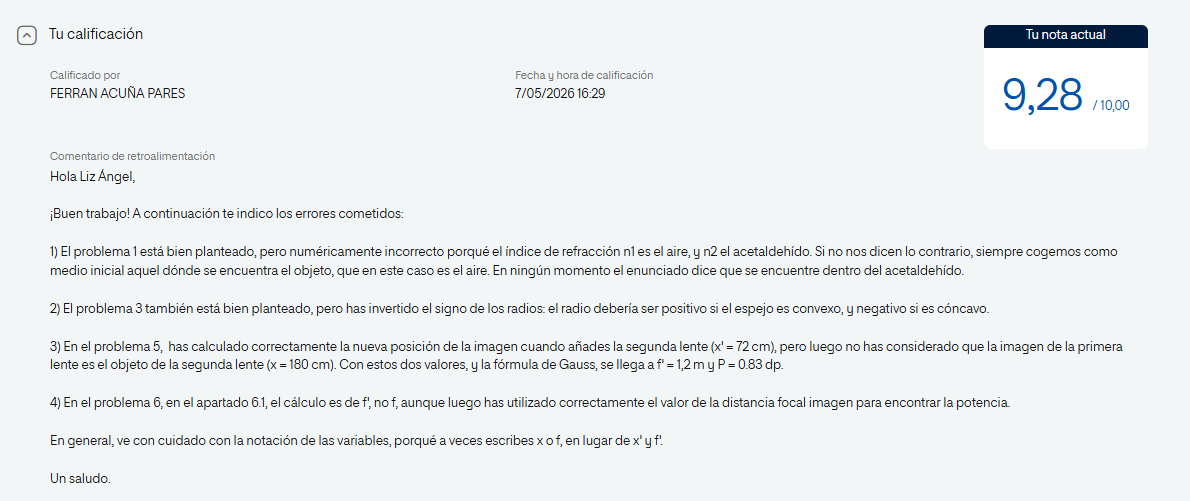
\includegraphics[width = 1.2 \textwidth]{correccion.png}
\end{figure}



\end{document}